\documentclass[12pt,letterpaper]{article}
\usepackage[utf8]{inputenc}
\usepackage[spanish]{babel}
\usepackage[T1]{fontenc}
\usepackage{bookman}
\usepackage{makeidx}
\usepackage{amsmath}
\usepackage{amsfonts}
\usepackage{amssymb}
\usepackage{listings}
\usepackage{cite}
\usepackage{graphicx}
\usepackage{subfig}
\usepackage{float}
\usepackage{ragged2e}
\graphicspath{ {imagenes/} }
\usepackage[left=2.5cm,right=2.5cm,top=3cm,bottom=3cm]{geometry}
\title{Reporte primer bloque de Programas}
\author{Javier Said Naranjo Miranda}

\begin{document}
\begin{titlepage}
\centering
	{\LARGE Instituto Polit\'ecnico Nacional \par}
	\vspace{1cm}
	{\Large Escuela Superior de C\'omputo \par}	
	\vspace{1.5cm}
	{\large Teor\'ia Computacional \par}
	\vspace{1cm}
	{\Large Reporte primer bloque de programas \par}
	\vspace{1.5cm}
	{\Large\itshape Alumno: Javier Said Naranjo Miranda \par}
	\vfill
	Grupo: 2CM4 \par
	\vfill	
	\newpage
	

\end{titlepage}
	
\raggedright
\tableofcontents
\newpage
	
\section{ Alfabeto}
\subsection{ Descripci\'on del programa}
\justify
El siguiente programa dado un alfabeto binario $\sum = \lbrace 0, 1 \rbrace $  calcula todas las palabras posibles que pueden ser formadas a partir de dicho alfabeto.\\
Es decir $\sum^{*} = \sum^{0}\cup{\sum}^{1}\cup{\sum}^{2}\cup\cdots\cup{\sum}^{n}$.\\
Este programa calculara a partir de una longitud de $0 \leq n \leq 1000$.
EL programa tendr\'a dos modos, el manual y el autom\'atico,en el primero el usuario elegir\'a la potencia a la cual quiere hacer las cadenas y si desea hacer un conteo nuevo, mientras que en el segundo se generara un numero aleatorio y de igual forma la opci\'on de nuevo conteo ser\'a aleatoria.Cada una de las palabras se guardara en un archivo de texto en ambos casos.\\
\subsection{C\'odigo}
EL lenguaje utilizado para la resoluci\'on del problema fue python.\\
El c\'digo utilizado para la resoluci\'on del problema se muestra a continuaci\'on:\\

C\'odigo: main.py
\lstset{language=Python, breaklines=true, basicstyle=\footnotesize}
\begin{lstlisting}[frame=single]
import cadenas

cadenas.iniciar_archivo()

opcion = cadenas.menu()

if (opcion == 1):
#Modo manual
	while True:
		tamanio = cadenas.tamanio()
		cadenas.iniciar_programa(tamanio)
		while True:
			op = cadenas.nuevo_conteo()
			if (op == 1):
				break
			elif (op == 2):
				exit()
			else:
				continue


elif(opcion == 2):
#Modo automatico
	while True:
		num = cadenas.num_aleatorio()
		print (num)
		cadenas.iniciar_programa(num)
		while True:
			opa=cadenas.opcion_aleatoria()
			print("1.-Nuevo conteo\n2.-salir ", opa)

			if (opa == 1):
				break
			elif (opa == 2):
				exit()
			else:
				continue

else:

	print("Introduce una opcion valida")
	exit()

\end{lstlisting}
\vspace{1.5cm}
C\'odigo:cadenas.py

\lstset{language=Python, breaklines=true, basicstyle=\footnotesize}
\begin{lstlisting}[frame=single]
import random
def menu():
	try:
		opcion = input("1.-Modo Manual\n2.-Modo Automatico ")
		opcion = int(opcion)
		return opcion
	except:
		print("Introduce una opcion valida")
def nuevo_conteo():
	try:
		conteo = input("1.-Nuevo conteo\n2.-salir ")
		conteo = int(conteo)
		return conteo
	except:
		print("opcion invalida")


def num_aleatorio():
	numero = random.randrange(1000)
	return numero
def opcion_aleatoria():
	opcion = random.randrange(1,3)
	return opcion

def iniciar_archivo ():
	try:
		archivo = open("cadenas.txt","w")
		archivo.close()
	except:
		exit()
def tamanio():
	try:
		tam = input("Introduce el tamanio de la cadena:")
		tam = int(tam)
		return tam
	except:
		print("No es un numero")
		exit()

def iniciar_programa(tamanio):
	cadena=['0','1']
	cad_aux=[]
	cont=0
	continuar = True

	archivo = open("cadenas.txt","a")
	archivo.write("S = { e")

	for indice in range (1,tamanio+1):
		print ("Va en ",indice)
		cad_aux = [0] * indice

		while continuar:
			archivo.write(", ")

			for i in range(indice):
				archivo.write(cadena[cad_aux[i]])
			cont = 0
			while (cont < indice):
				cad_aux[cont]=cad_aux[cont] + 1
				if (cad_aux[cont] > 1):
					cad_aux[cont] = 0
				else:
					break
				cont = cont +1
			if (cont>=indice):
				cad_aux=[]
				break
	archivo.write(" }\n")
	archivo.close() 


\end{lstlisting}
\newpage
\subsection{Pruebas}
A continuaci\'on se mostraran algunas im\'agenes capturadas al momento de ejecutar el programa, dichas im\'agenes mostraran los resultados obtenidos.\\
\vspace{1.0cm}
Para el modo manual:\\
\begin{figure}[H]
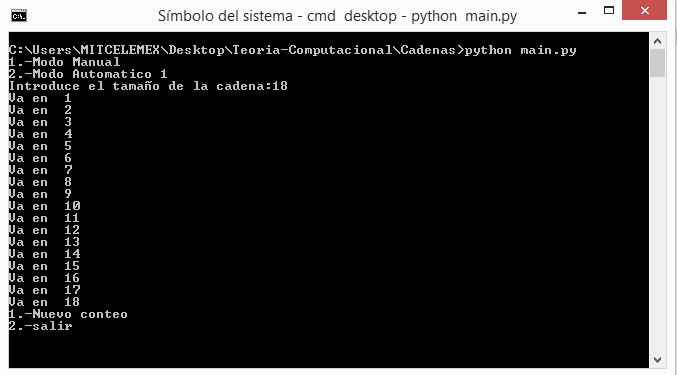
\includegraphics[width=\textwidth, height=7cm]{modomanualinicio.png}
\label{fig:manual_alfabeto}
\caption{Selecci\'on de un tama\~no de 18 introducido de forma manual}
\end{figure}

\begin{figure}[H]
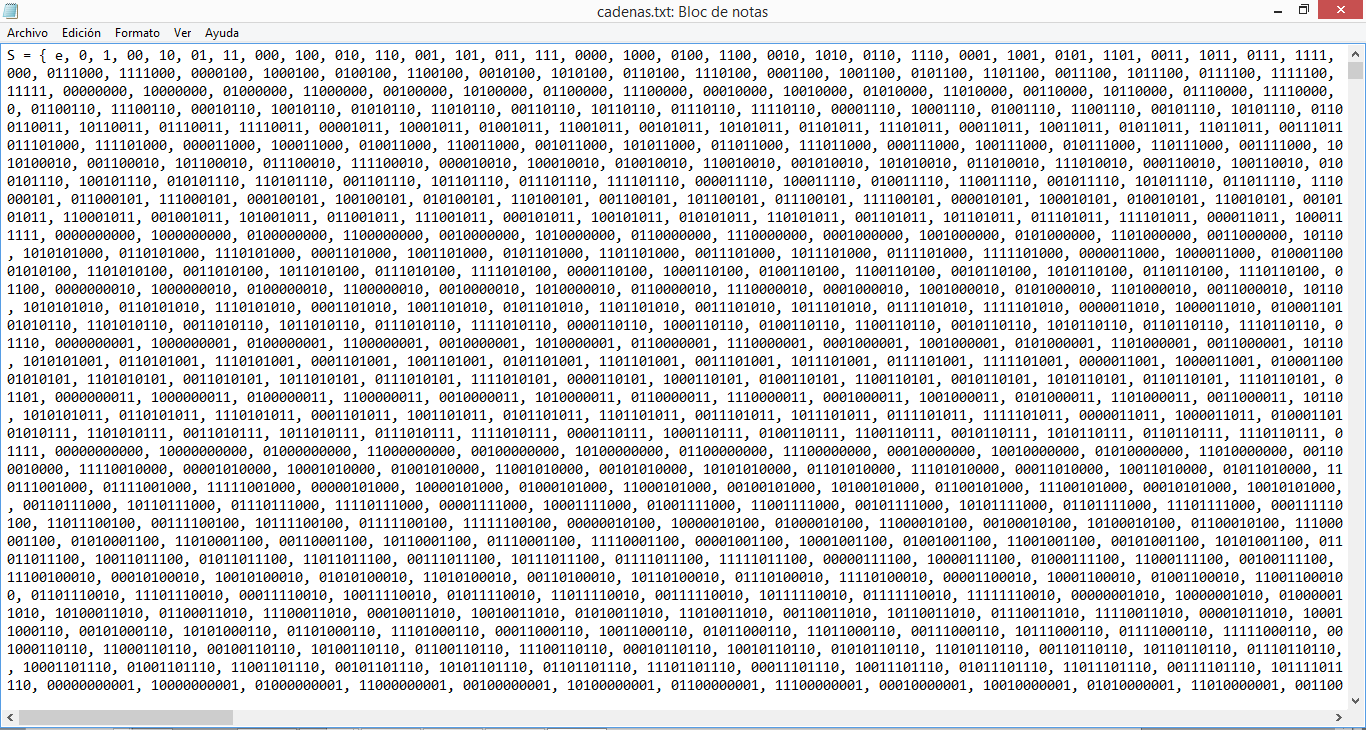
\includegraphics[width=\textwidth, height=7cm]{textomodomanual.png}
\label{fig:manualtexto_alfabeto}
\caption{Parte del texto de las cadenas producidos para un tama\~no de 18}
\end{figure}

\begin{figure}[H]
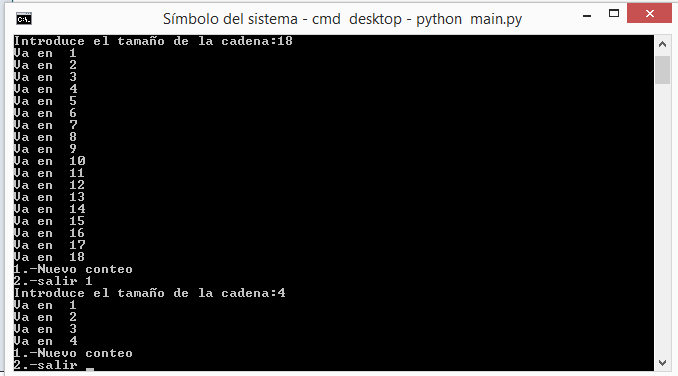
\includegraphics[width=\textwidth, height=7cm]{nuevoconteo.png}
\label{fig:manualnuevoconteo_alfabeto}
\caption{Nuevo conteo de tama\~no 4}
\end{figure}

Para el modo autom\'atico:\\
\begin{figure}[H]
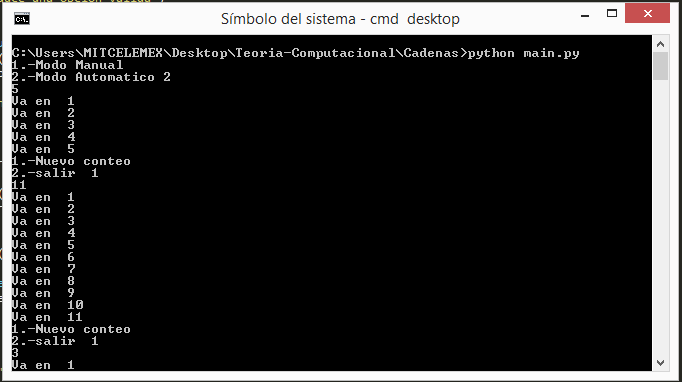
\includegraphics[width=\textwidth, height=7cm]{modoautomatico.png}
\label{fig:auto_alfabeto}
\caption{Selecci\'on del modo autom\'atico con un tama\~no de 5 y posteriormente un nuevo conteo con un tama\~no de 11}
\end{figure}

\begin{figure}[H]
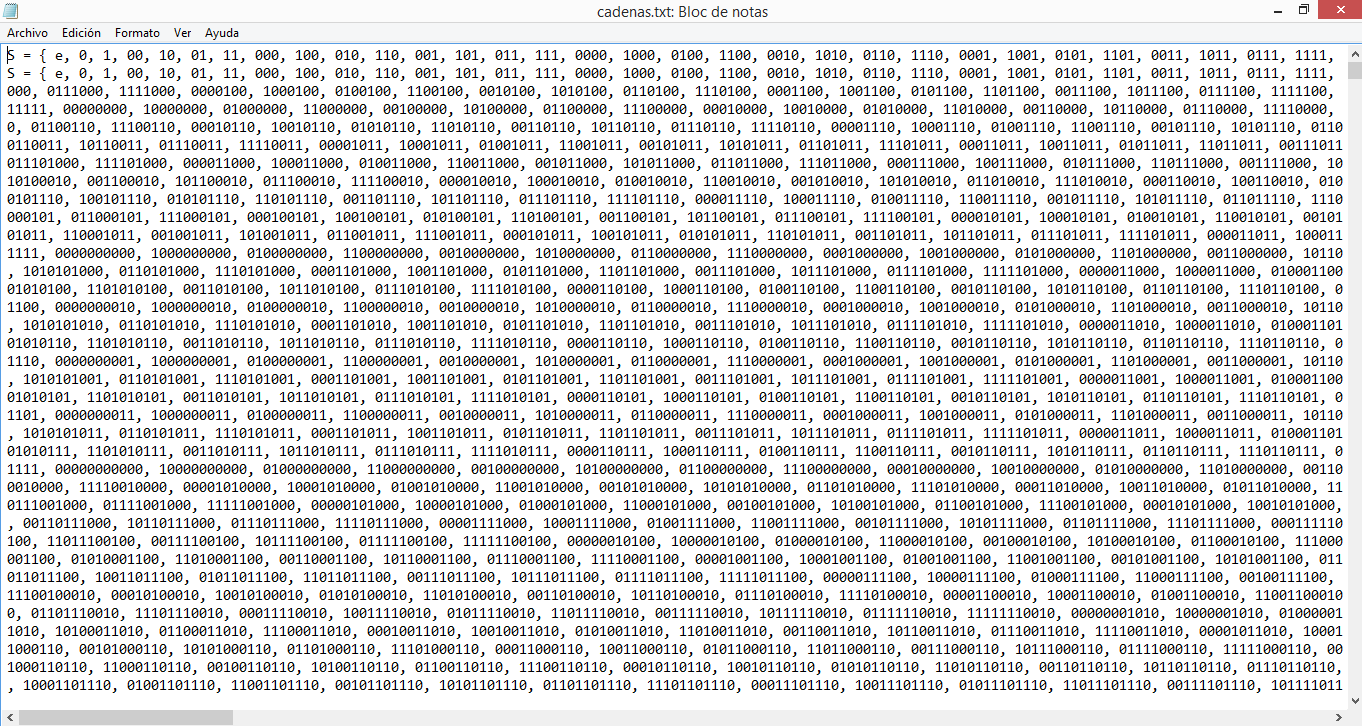
\includegraphics[width=\textwidth, height=7cm]{textoautomatico.png}
\label{fig:autotexto_alfabeto}
\caption{Parte del texto de las cadenas obtenidas por el modo autom\'atico}
\end{figure}
\newpage
\section{N\'umeros primos}
\subsection{Descripci\'on}
\justify
El siguiente programa calcula todos los n\'umeros primos que se encuentran por debajo del limite que se establezca, cabe resaltar que un n\'umero primo es aquel que solo puede ser dividido entre si mismo y entre 1.Actualmente no existe un m\'etodo directo para calcular todos los n\'umeros primos\\
El programa har\'a un calculo que tendr\'a como un limite m\'aximo el numero 1000\\
El programa tendr\'a dos modos, el manual y el autom\'atico, en el primero el usuario elegir\'a el numero m\'aximo y si desea calcular los n\'umeros de nuevo, mientras que en el manual todo se har\'a por medio de numero aleatorios. En ambos casos se guardara en un archivo los n\'umeros primos encontrados as\'i como su conversi\'on a n\'umero binario.\\
\subsection{C\'odigo}
\justify
EL lenguaje utilizado para la resoluci\'on del problema fue python.\\
El c\'digo utilizado para la resoluci\'on del problema se muestra a continuaci\'on:\\

C\'odigo: mainNP.py
\lstset{language=Python, breaklines=true, basicstyle=\footnotesize}
\begin{lstlisting}[frame=single]
import primos
primos.iniciar_archivo()

opcion = primos.menu()

if (opcion == 1):
#Modo manual
	while True:
		numero = primos.numero()
		primos.iniciar_programa(numero)
		
		while True:
			op = primos.nuevo_conteo()
			if (op == 1):
				break
			elif (op == 2):
				exit()
			else:
				continue
# modo automarico
elif(opcion == 2):
	while True:
		numero = primos.num_aleatorio()
		primos.iniciar_programa(numero)
		while True:
			op = primos.opcion_aleatoria()
			print("1.-Nuevo conteo\n2.-salir ")
			if (op == 1):
				break
			elif(op==2):
				exit()
			else:
				continue

\end{lstlisting}
\vspace{1.5cm}
C\'odigo:primos.py
\lstset{language=Python, breaklines=true, basicstyle=\footnotesize}
\begin{lstlisting}[frame=single]
import random

def menu():
	try:
		
			opcion = input("1.-Modo Manual\n2.-Modo Automatico ")
			opcion = int(opcion)
			return opcion
	except:
		print("Introduce una opcion valida")
def nuevo_conteo():
	try:
		conteo = input("1.-Nuevo conteo\n2.-salir ")
		conteo = int(conteo)
		return conteo
	except:
		print("opcion invalida")


def num_aleatorio():
	numero = random.randrange(1,1001)
	return numero
def opcion_aleatoria():
	opcion = random.randrange(1,3)
	return opcion
def iniciar_archivo():
	try:
		archivo = open("numprimo.txt","w")
		archivo.close
	except:
		exit()
def numero():
	try:
		num = input("Introduce un numero: ")
		num = int(num)
		return num
	except:
		print("No es un numero")
		exit()

def iniciar_programa(numero):
	archivo = open("numprimo.txt","a")

	primos = [2,3,5,7,11]
	binario = []	
	obtener_primos(primos,binario,archivo,numero)
	escribir_archivo_binario(archivo,binario)
	print("numero de ceros")
	contar_ceros(binario)
	print("numero de unos")
	contar_unos(binario)
	archivo.close()

def obtener_primos(primos,binario,archivo,numero):
	archivo.write("{ ")
	if (numero >= 2):
		for numero in range(2,numero+1):
			cont=0
			for valor in primos:
				if (numero == valor):
					archivo.write(str(numero)+", ")
					binario.append(bin(numero))
					break
				else:
					mod = numero % valor
					if(mod == 0):
						break
					else:
						if(cont<len(primos)):
							cont = cont +1
							if (cont == (len(primos)-1)):
								primos.append(numero)
								archivo.write(str(numero))
								archivo.write(", ")
								binario.append(bin(numero))
								break
							else: 
								continue

		archivo.write(" }\n")
			
	else:
		print("no tiene numeros primos")

def escribir_archivo_binario(archivo,binario):
	archivo.write("{ ")
	for num_bin in binario:
		archivo.write(str(num_bin)+",")
	archivo.write("}\n")

def contar_ceros(binario):
	for bin in binario:
		bin = str(bin)
		print((bin.count("0"))-1)

def contar_unos(binario):
	for bin in binario:
		bin = str(bin)
		print(bin.count("1"))
\end{lstlisting}
\newpage
\subsection{Pruebas}
A continuaci\'on se mostraran algunas im\'agenes capturadas al momento de ejecutar el programa, dichas im\'agenes mostraran los resultados obtenidos.\\

Para el modo manual:\\
\begin{figure}[H]
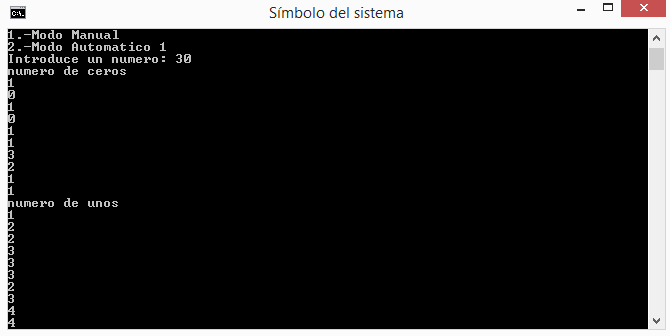
\includegraphics[width=\textwidth, height=7cm]{modomanualprimo.png}
\label{fig:manual_primo}
\caption{Selecci\'on de un n\'umero limite de 30}
\end{figure}
\begin{figure}[H]
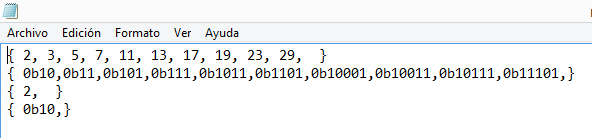
\includegraphics[width=\textwidth, height=7cm]{textomanualprimo.png}
\label{fig:manualtexto_primo}
\caption{Salida en archivo de texto del modo manual}
\end{figure}
Para el modo Autom\'atico:\\

\begin{figure}[H]
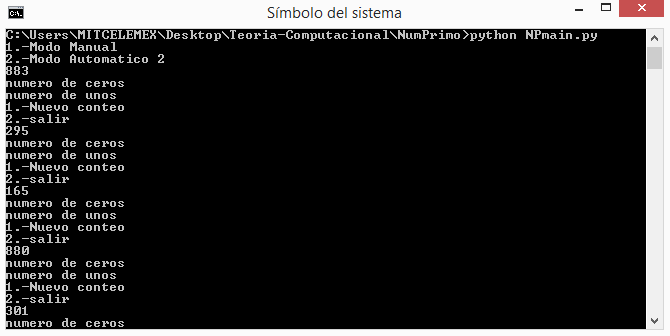
\includegraphics[width=\textwidth, height=7cm]{automaticoprimo.png}
\label{fig:automatico_primo}
\caption{Ejecuci\'on del modo autom\'atico}
\end{figure}

\begin{figure}[H]
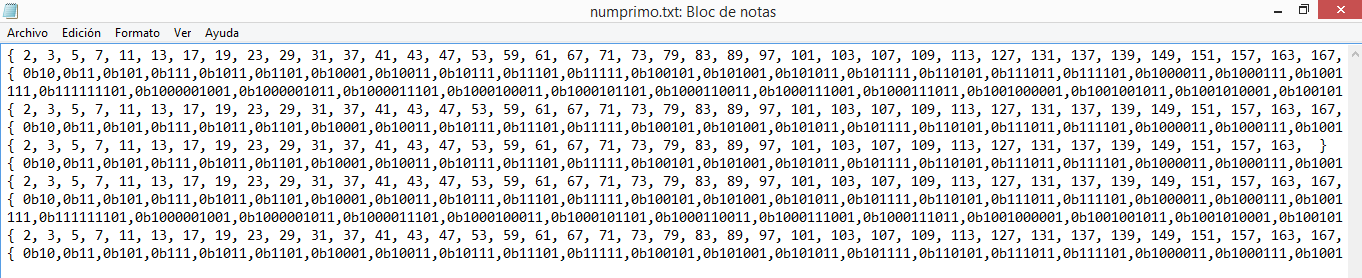
\includegraphics[width=\textwidth, height=7cm]{textoautomaticoprimo.png}
\label{fig:automaticotexto_primo}
\caption{Parte de la salida de texto del modo autom\'atico}
\end{figure}

Se realizo una gr\'afica en la cual se puede visualizar la relacion entre 1's y 0's de cada n\'umero primo.

\begin{figure}[H]
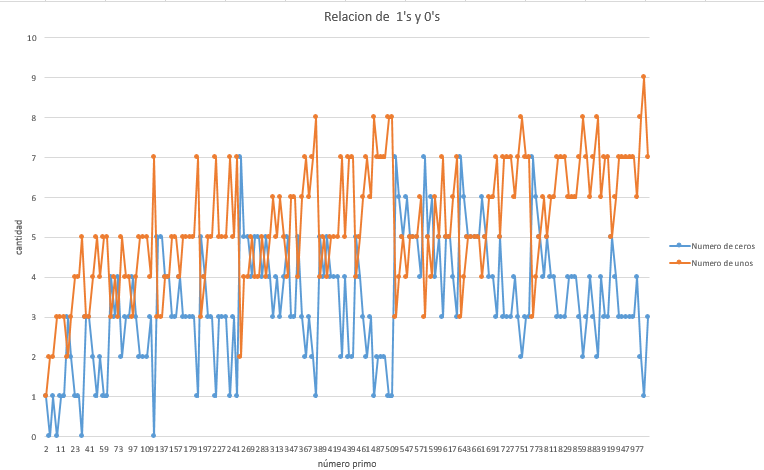
\includegraphics[width=\textwidth, height=7cm]{graficaprimo.png}
\label{fig:grafica_primo}
\caption{Gr\'afica de la relaci\'on entre 1's y 0's de cada n\'umero primo.}
\end{figure}
\newpage
\section{Palabras terminadas con ere(Aut\'omata)}
\subsection{Descripci\'on}
\justify
El siguiente aut\'omata reconocer\'a todas las palabras terminadas con ere, este aut\'omata podr\'a reconocer las palabras terminadas con ere de textos en ingl\'es y en espa\~nol, de este ultimo siempre y cuando no tengan acentos.\\
El aut\'omata tendr\'a un modo para introducir un texto de manera manual y otro para leer un archivo, este devolver\'a en pantalla las palabras encontradas as\'i como en que posici\'on se encuentran.\\
El aut\'omata utilizado para modelar el problemas es el siguiente:
\begin{figure}[H]
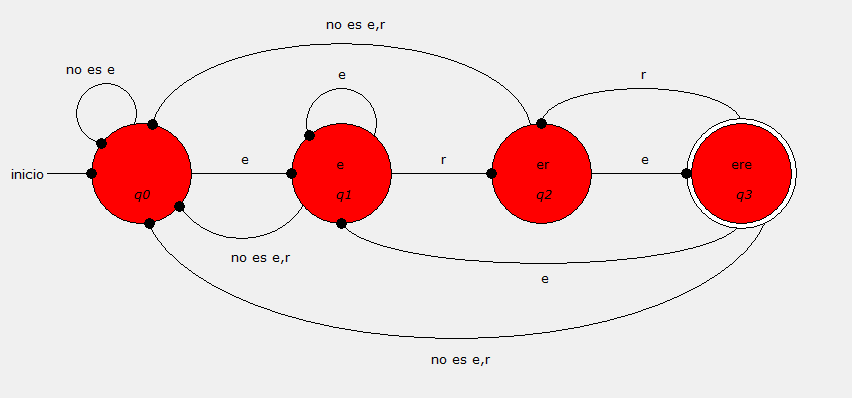
\includegraphics[width=\textwidth, height=7cm]{diagramaautomata.png}
\label{fig:automataere}
\caption{Aut\'omata.}
\end{figure}

\subsection{C\'odigo}
Se mostrara el c\'odigo del gr\'afico del aut\'omata\\
C\'odigo:Diagrama1.py
\lstset{language=Python, breaklines=true, basicstyle=\footnotesize}
\begin{lstlisting}[frame=single]
from tkinter import *

def crearDiagrama():
	ventana =  Tk()
	ventana.geometry("900x500")  #geometry(widthxheight)
	ventana.title("Automata ERE")
	ventana.resizable(width=False,height=False)
	AreaDibujo=Canvas(ventana,width=890,height=490)
	AreaDibujo.pack()

	#Creacion de arcos para transicion
	AreaDibujo.create_arc(315,115,385,185,start=-25,extent=250)
	AreaDibujo.create_arc(550,115,750,185,start=8,extent=180,style=ARC)
	AreaDibujo.create_arc(350,200,750,290,start=180,extent=168,style=ARC)
	AreaDibujo.create_arc(180,140,320,265,start=180,extent=168,style=ARC)
	AreaDibujo.create_arc(160,70,540,250,start=-20,extent=210,style=ARC)
	AreaDibujo.create_oval(85,110,145,170)
	AreaDibujo.create_arc(150,75,780,365,start=180,extent=180,style=ARC)

	

	#Creacion de Circulos de estado
	AreaDibujo.create_oval(695,145,805,255,fill="white")
	AreaDibujo.create_oval(100,150,200,250,fill="red")
	AreaDibujo.create_oval(300,150,400,250,fill="red")
	AreaDibujo.create_oval(500,150,600,250,fill="red")
	AreaDibujo.create_oval(700,150,800,250,fill="red")
	
	#Creacion de circulo de referencia


	AreaDibujo.create_oval(95,195,105,205,fill="black")
	AreaDibujo.create_oval(295,195,305,205,fill="black")
	AreaDibujo.create_oval(495,195,505,205,fill="black")
	AreaDibujo.create_oval(690,195,700,205,fill="black")
	AreaDibujo.create_oval(313,157,323,167,fill="black")
	AreaDibujo.create_oval(545,145,555,155,fill="black")
	AreaDibujo.create_oval(345,245,355,255,fill="black")
	AreaDibujo.create_oval(105,165,115,175,fill="black")
	AreaDibujo.create_oval(156,146,166,156,fill="black")
	AreaDibujo.create_oval(183,228,193,238,fill="black")
	AreaDibujo.create_oval(153,245,163,255,fill="black")

	#Creacion de lineas para transicion

	AreaDibujo.create_line(50,200,100,200)
	AreaDibujo.create_line(200,200,300,200)
	AreaDibujo.create_line(400,200,500,200)
	AreaDibujo.create_line(600,200,700,200)


	#Creacion de etiquetas

	#estados
	inicio=Label(ventana,text="inicio",font="Verdana 10 roman").place(x=20,y=190)
	qo=Label(ventana,text="q0",background="red",font="Verdana 10 italic").place(x=143,y=210)
	q1=Label(ventana,text="q1",background="red",font="Verdana 10 italic").place(x=345,y=210)
	q2=Label(ventana,text="q2",background="red",font="Verdana 10 italic").place(x=545,y=210)
	q3=Label(ventana,text="q3",background="red",font="Verdana 10 italic").place(x=745,y=210)

	qoe=Label(ventana,text="e",background="red",font="Verdana 10 roman").place(x=345,y=180)
	qo=Label(ventana,text="er",background="red",font="Verdana 10 roman").place(x=545,y=180)
	qo=Label(ventana,text="ere",background="red",font="Verdana 10 roman").place(x=740,y=180)

	#transiciones
	letra_e=Label(ventana,text="e",font="Verdana 10 roman").place(x=250,y=175)
	letra_r=Label(ventana,text="r",font="Verdana 10 roman").place(x=450,y=175)
	letra_eFinal=Label(ventana,text="e",font="Verdana 10 roman").place(x=650,y=175)
	letra_eQ0=Label(ventana,text="e",font="Verdana 10 roman").place(x=347,y=90)
	letra_rQ3Q2=Label(ventana,text="r",font="Verdana 10 roman").place(x=650,y=90)
	letra_eQ3Q1=Label(ventana,text="e",font="Verdana 10 roman").place(x=550,y=294)
	noes_e=Label(ventana,text="no es e",font="Verdana 10 roman").place(x=75,y=85)
	noes_er=Label(ventana,text="no es e,r",font="Verdana 10 roman").place(x=440,y=375)
	noes_er=Label(ventana,text="no es e,r",font="Verdana 10 roman").place(x=335,y=40)
	noes_er=Label(ventana,text="no es e,r",font="Verdana 10 roman").place(x=240,y=273)

	ventana.mainloop()


\end{lstlisting}
\vspace{1cm}

C\'odigo:main.py
\lstset{language=Python, breaklines=true, basicstyle=\footnotesize}
\begin{lstlisting}[frame=single]
import automata
import funciones
import Diagrama1



while True:
	fila=[]
	palabra=[]
	try:
		opcion=input('1.-Introducir Texto\n2.-Leer un texto\n3.-Grafico del automata\nElige una opcion: ')
		opcion=int(opcion)
	except:
		print("Introduce una opcion valida")
		continue

	if (opcion==1):
		texto=funciones.texto()
		palabras = automata.automata_ere(texto,fila,palabra)
		funciones.imprimir_palabras_ere(palabras,fila,palabra)
		funciones.nuevo_texto()

	elif(opcion==2):
		texto=funciones.leer_archivo()
		palabras = automata.automata_ere(texto,fila,palabra)
		funciones.imprimir_palabras_ere(palabras,fila,palabra)
		funciones.nuevo_texto()
	elif(opcion==3):
		Diagrama1.crearDiagrama()
		

	else:
		print('Introduce una opcion valida')
		continue

\end{lstlisting}
\vspace{1cm}

C\'odigo:funciones.py
\lstset{language=Python, breaklines=true, basicstyle=\footnotesize}
\begin{lstlisting}[frame=single]
import tkinter as tk
def texto():
	texto=input('Introduce un texto\n')
	return texto
def nuevo_texto():
	while True:
			try:
				seguir=input('1.-Si\n2.-No\nDesea iniciar el automata de nuevo: ')
				seguir=int(seguir)
			except:
				print('Introduce una opcion valida')
				continue
			if(seguir==1):
				break
			elif(seguir==2):
				exit()
			else:
				continue

def imprimir_palabras_ere(palabras,fila,palabra):
	i=0
	for pala in palabras:
		fil=fila[i]
		fil=str(fil)
		pal=palabra[i]
		pal=str(pal)
		print("Palabra: " + pala+" fila: "+fil+" palabra numero: "+pal)
		i=i+1

def leer_archivo():
	archivo=open("archivo.txt","r")
	lineas=str(archivo.read())
	archivo.close()
	return lineas

\end{lstlisting}
\vspace{1cm}

C\'odigo:automata.py
\lstset{language=Python, breaklines=true, basicstyle=\footnotesize}
\begin{lstlisting}[frame=single]
def automata_ere(texto,fila,palabra):
	estado=0
	palabras_ere=[]
	auxiliar_palabra = ''
	contfilas=1
	contpalabra=1

	for caracter in texto:
		
		aux_caracter = caracter.lower()

		if (estado ==0):
			estado = estadoCero(aux_caracter)
		elif(estado==1):
			estado= estadoUno(aux_caracter)
		elif(estado==2):
			estado= estadoDos(aux_caracter)
		elif(estado==3):
			estado= estadoTres(aux_caracter)

		if(ord(aux_caracter)>=97 and ord(aux_caracter)<=122):
			auxiliar_palabra = auxiliar_palabra + aux_caracter
			if (estado==-1):
				estado =0
				auxiliar_palabra=''
		else:
			if(estado ==-1):
				palabras_ere.append(auxiliar_palabra)
				fila.append(contfilas)
				palabra.append(contpalabra)
				auxiliar_palabra=''
				estado=0	
			else:
				estado=0
				auxiliar_palabra = ''
		if(caracter==" " ):
			contpalabra=contpalabra+1
		if(caracter=="\n"):
			contfilas=contfilas+1
			contpalabra=1
	if(estado==3):
		palabras_ere.append(auxiliar_palabra)
		fila.append(contfilas)
		palabra.append(contpalabra)

	return palabras_ere

def estadoCero(caracter):
	if(caracter =='e'):
		print('Q0--->Q1')
		return 1
	else:
		print('Q0--->Q0')
		return 0
	
def estadoUno(caracter):
	if(caracter == 'e'):
		print('Q1--->Q1')
		return 1
	elif(caracter == 'r'):
		print('Q1--->Q2')
		return 2
	else:
		print('Q1--->Q0')
		return 0

def estadoDos(caracter):
	if(caracter == 'e'):
		print('Q2--->Q3')
		return 3
	else:
		print('Q2--->Q0')
		return 0
	
def estadoTres(caracter):
	if(caracter == 'r'):
		print('Q3--->Q2')
		return 2
	elif(caracter == 'e'):
		print('Q3--->Q1')
		return 1
	else:
		return -1


#ASCII letras minusculas 97-122
\end{lstlisting}
\vspace{1cm}
\newpage 
\subsection{Pruebas}
Se mostraran algunas pruebas realizadas de los modos manual, leer archivo y mostrar diagrama.\\
Para el modo manual en el que se introducir\'a una cadena.
\begin{figure}[H]
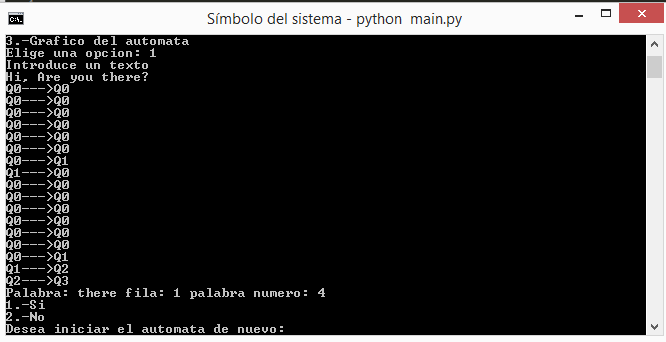
\includegraphics[width=\textwidth, height=8cm]{manualERE.png}
\label{fig:manualautomataere}
\caption{Modo manual en el cual se introdujo una cadena}
\end{figure}

Para el modo leer archivo.En este modo el archivo que se leera sera la biografia de William Shakespeare[1]\\

\begin{figure}[H]
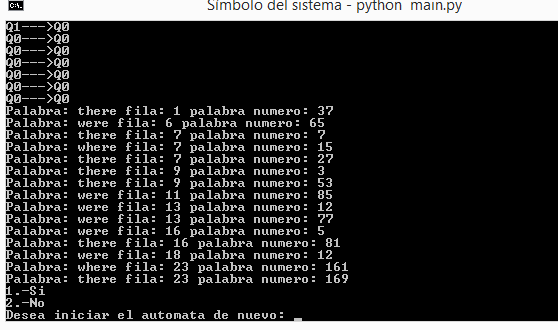
\includegraphics[width=\textwidth, height=8cm]{leerERE.png}
\label{fig:leerautomataere}
\caption{Modo leer archivo}
\end{figure}

\begin{figure}[H]
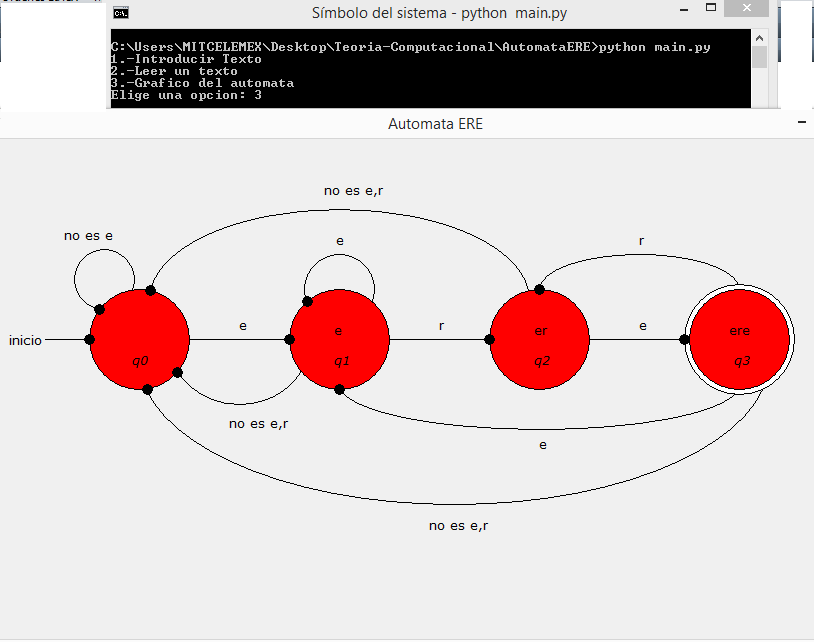
\includegraphics[width=\textwidth, height=9cm]{diagERE.png}
\label{fig:Diagautomataere}
\caption{Visualizar diagrama del aut\'omata}
\end{figure}


\newpage
\section{Aut\'omata Paridad}
\subsection{Descripci\'on}
\justify
El siguiente programa determina si una cadena binaria tiene paridad de 1's y 0', es decir tiene una cantidad par de 1's y una cantidad par de 0's\\
El programa tendr\'a dos modos, el modo manual y autom\'atico, en el modo manual el usuario ingresara una cadena binaria de la longitud deseada, el modo autom\'atico generara una cadena binaria con una cardinalidad de entre 1 a 1000,en ambos casos se mostrara en pantalla si la cadena tiene o no paridad.\\
De igual forma se podr\'a observar el diagrama del aut\'omata.\\
El aut\'omata a utilizar es el siguiente:\\

\begin{figure}[H]
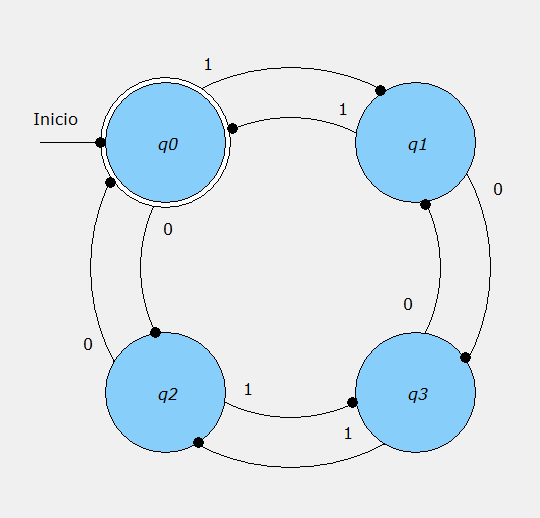
\includegraphics[width=\textwidth, height=7cm]{diagramaautomataPar.png}
\label{fig:automataParidad}
\caption{Aut\'omata.}
\end{figure}

\subsection{C\'odigo}
Se mostrara el c\'odigo del diagrama de paridad\\
C\'odigo:Diagrama2.py
\lstset{language=Python, breaklines=true, basicstyle=\footnotesize}
\begin{lstlisting}[frame=single]
from tkinter import *

def mostarDiagrama():
	ventana1 = Tk()
	ventana1.geometry("600x600+400+50")  #geometry(widthxheight)
	ventana1.title("Automata Paridad")
	ventana1.resizable(width=False,height=False)
	AreaDibujo1=Canvas(ventana1,width=595,height=595)
	AreaDibujo1.pack()

	#Circulos transicion
	AreaDibujo1.create_oval(100,100,500,500)
	AreaDibujo1.create_oval(150,150,450,450)


	#Circulos de estado
	AreaDibujo1.create_oval(110,110,240,240,fill="white")
	AreaDibujo1.create_oval(115,115,235,235,fill="light sky blue")
	AreaDibujo1.create_oval(365,115,485,235,fill="light sky blue")
	AreaDibujo1.create_oval(115,365,235,485,fill="light sky blue")
	AreaDibujo1.create_oval(365,365,485,485,fill="light sky blue")

	#Linea de inicio
	AreaDibujo1.create_line(50,175,110,175)

	#Circulos de sentido
	AreaDibujo1.create_oval(105,170,115,180, fill="black")
	AreaDibujo1.create_oval(385,118,395,128,fill="black")
	AreaDibujo1.create_oval(470,385,480,395,fill="black")
	AreaDibujo1.create_oval(203,470,213,480,fill="black")
	AreaDibujo1.create_oval(115,210,125,220,fill="black")

	AreaDibujo1.create_oval(237,156,247,166,fill="black")
	AreaDibujo1.create_oval(160,360,170,370,fill="black")
	AreaDibujo1.create_oval(357,430,367,440,fill="black")
	AreaDibujo1.create_oval(430,232,440,242,fill="black")

	#etiquetas
	inicio=Label(ventana1,text="Inicio",font="Verdana 12 roman").place(x=40,y=140)
	qo=Label(ventana1,text="q0",font="Verdana 12 italic",background="light sky blue").place(x=165,y=165)
	q1=Label(ventana1,text="q1",font="Verdana 12 italic",background="light sky blue").place(x=415,y=165)
	q2=Label(ventana1,text="q2",font="Verdana 12 italic",background="light sky blue").place(x=165,y=415)
	q3=Label(ventana1,text="q3",font="Verdana 12 italic",background="light sky blue").place(x=415,y=415)

	#etiquetas transicion
	qoq1=Label(ventana1,text="1",font="Verdana 12 roman").place(x=210,y=85)
	q1q0=Label(ventana1,text="1",font="Verdana 12 roman").place(x=345,y=130)

	q2q3=Label(ventana1,text="1",font="Verdana 12 roman").place(x=250,y=410)
	q3q2=Label(ventana1,text="1",font="Verdana 12 roman").place(x=350,y=454)

	qoq2=Label(ventana1,text="0",font="Verdana 12 roman").place(x=170,y=250)
	q2qo=Label(ventana1,text="0",font="Verdana 12 roman").place(x=90,y=365)

	q1q3=Label(ventana1,text="0",font="Verdana 12 roman").place(x=500,y=210)
	q3q1=Label(ventana1,text="0",font="Verdana 12 roman").place(x=410,y=325)

	ventana1.mainloop()

\end{lstlisting}
\vspace{1 cm}
C\'odigo:mainPar.py
\lstset{language=Python, breaklines=true, basicstyle=\footnotesize}
\begin{lstlisting}[frame=single]
import automataPar
import Diagrama2
import funcionesPar


#menu
opcion=funcionesPar.menu()


if(opcion==1):
	while True:
		
		cadena=input("Introduce una cadena binaria: ")
		print(cadena)
		print("numero de ceros: " + str(cadena.count("0")))
		print("numero de unos: " + str(cadena.count("1")))

		
		resultado=automataPar.automata(cadena)
		if(resultado==1):
			print("Es una cadena con paridad")
		elif(resultado==0):
			print("No es una cadena con paridad")
		else:
			print("no es una cadena binaria")
		while True:
			nC=funcionesPar.nueva_cadena()
			if(nC==1):
				break
			elif(nC==2):
				exit()
			else:
				continue

elif(opcion==2):
	while True:
		
		cadena=funcionesPar.generarCadena()
		print(cadena)
		print("numero de ceros: " + str(cadena.count("0")))
		print("numero de unos: " + str(cadena.count("1")))
		resultado=automataPar.automata(cadena)
		if(resultado==1):
			print("Es una cadena con paridad")
		elif(resultado==0):
			print("No es una cadena con paridad")
		
		while True:
			print("1.-Nuevo conteo\n2.-salir ")
			nC=funcionesPar.op_aleatorio()
			if(nC==1):
				break
			elif(nC==2):
				exit()
			else:
				continue

elif(opcion==3):
	Diagrama2.mostarDiagrama()

else:
	print("opcion invalida")
\end{lstlisting}
\vspace{1 cm}

C\'odigo:funcionesPar.py
\lstset{language=Python, breaklines=true, basicstyle=\footnotesize}
\begin{lstlisting}[frame=single]
import random

def menu():
	try:
		opcion=input("\t\t Paridad\n1.-Modo manual\n2.-Modo Automatico\n3.-Mostrar Diagrama\nElige una opcion: ")
		opcion=int(opcion)
		return opcion
	except:
		exit()
def nueva_cadena():
	try:
		conteo = input("1.-Nuevo conteo\n2.-salir ")
		conteo = int(conteo)
		return conteo
	except:
		print("opcion invalida")

def generarCadena():
	cardinalidad=cardinalidad_aleatoria()
	tamanio=0
	cadena=""
	while (tamanio<cardinalidad):
		num=num_aleatorio()
		num=str(num)
		cadena=cadena+num
		tamanio=tamanio + 1
	return cadena



def cardinalidad_aleatoria():
	numero = random.randrange(1,1000)
	return numero
def num_aleatorio():
	bit = random.randrange(0,2)
	return bit
def num_aleatorio():
	bit = random.randrange(0,2)
	return bit
	
\end{lstlisting}
\vspace{1 cm}

C\'odigo:automataPar.py
\lstset{language=Python, breaklines=true, basicstyle=\footnotesize}
\begin{lstlisting}[frame=single]
#codigo ascii del 0-1   "48-49"
def automata(cadena):
	estado=0

	for bit in cadena:
		if(bit ==" "):
			break
		if(estado==0):
			estado=estadoCero(bit)
		elif(estado==1):
			estado=estadoUno(bit)
		elif(estado==2):
			estado=estadoDos(bit)
		elif(estado==3):
			estado=estadoTres(bit)
		
		

	if(estado==0):
		return 1
	elif(estado==-1):
		return -1
	else:
		return 0


def estadoCero(elemento):
	if(elemento=="0"):
		print("Q0 -- %s -->Q2" %elemento)
		return 2
	elif(elemento=="1"):
		print("Q0 -- %s -->Q1" %elemento)
		return 1
	else:
		return -1
def estadoUno(elemento):
	if (elemento=="0"):
		print("Q1 -- %s -->Q3" %elemento)
		return 3
	elif(elemento=="1"):
		print("Q1 -- %s -->Q0" %elemento)
		return 0
	else:
		return -1

	
def estadoDos(elemento):
	if(elemento=="0"):
		print("Q2 -- %s -->Q0" %elemento)
		return 0
	elif(elemento=="1"):
		print("Q2 -- %s -->Q3" %elemento)
		return 3
	else:
		return -1

def estadoTres(elemento):
	if(elemento=="0"):
		print("Q3 -- %s -->Q1" %elemento)
		return 1
	elif(elemento=="1"):
		print("Q3 -- %s -->Q2" %elemento)
		return 2
	else:
		return -1

\end{lstlisting}
\newpage
\subsection{Pruebas}
A continuaci\'on se mostraran las pruebas del programa.\\
Pruebas del modo manual.\\
\begin{figure}[H]
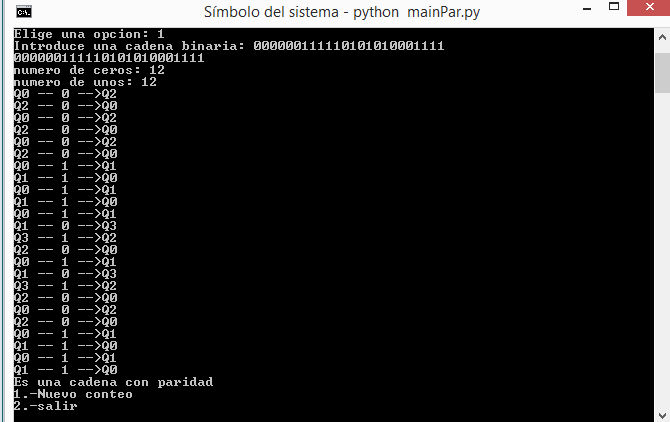
\includegraphics[width=\textwidth, height=7cm]{manualParidad.png}
\label{fig:manualparidad}
\caption{Modo manual al introducir una cadena binaria}
\end{figure}
\begin{figure}[H]
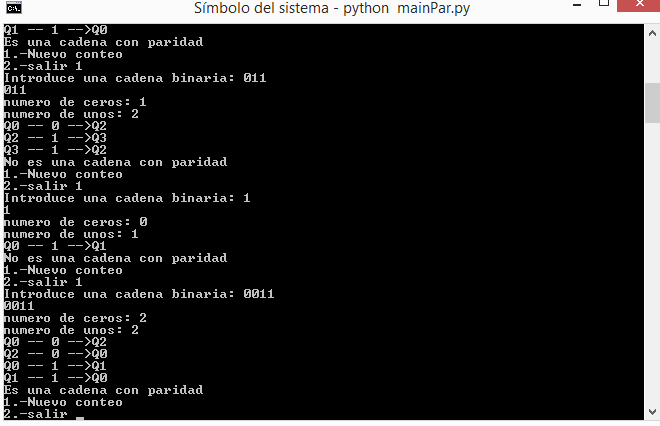
\includegraphics[width=\textwidth, height=7cm]{manualnuevaParidad.png}
\label{fig:manualnuevoparidad}
\caption{Modo manual al introducir una nueva cadena}
\end{figure}

Pruebas del modo autom\'atico.\\

\begin{figure}[H]
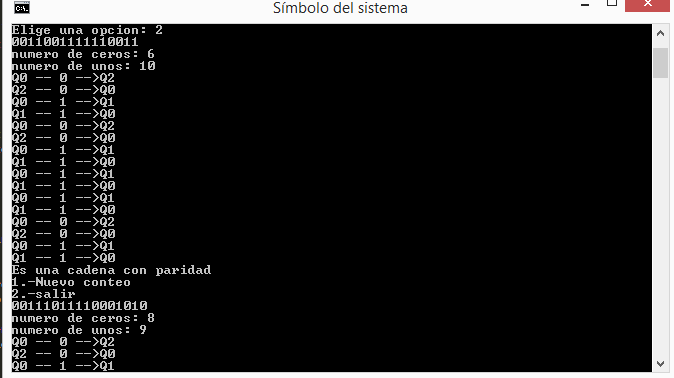
\includegraphics[width=\textwidth, height=7cm]{automaticoParidad.png}
\label{fig:automaticoparidad}
\caption{Modo autom\'atico generando cadena aleatoria}
\end{figure}

Prueba de la visualizaci\'on del diagrama.\\
\begin{figure}[H]
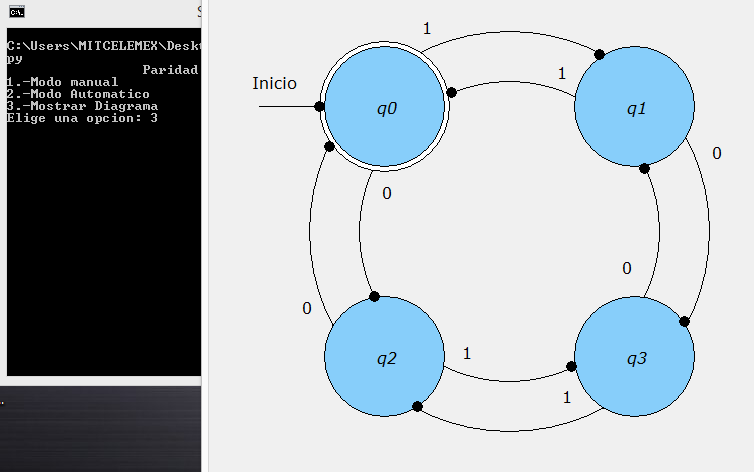
\includegraphics[width=\textwidth, height=9cm]{diagramaParidad.png}
\label{fig:Diaparidad}
\caption{Ejecuci\'on del diagrama desde el programa}
\end{figure}
\newpage
\section{Protocolo}
\subsection{Descripci\'on}
Se mostrara el funcionamiento de un protocolo, el siguiente programa generara un archivo con 50 cadenas binarias aleatorias, posteriormente se esperara un segundo de time out para posteriormente ser validadas por medio del aut\'omata de paridad, as\'i despu\'es se preguntara el estado del protocolo y si esta encendido se realizara lo antes dicho, de lo contrario acabara el programa.
Diagrama del protocolo\\
\begin{figure}[H]
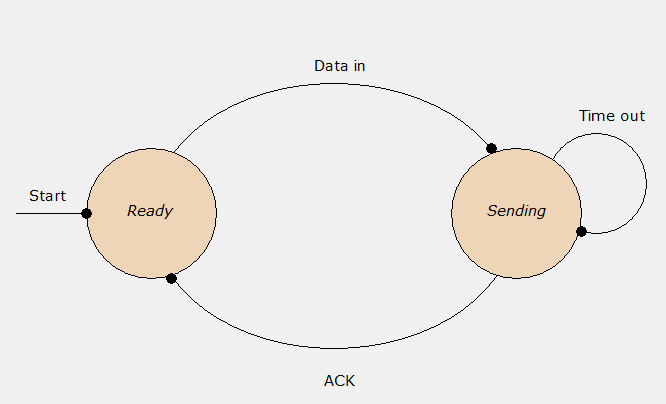
\includegraphics[width=\textwidth, height=9cm]{diagramaProtocolo.png}
\label{fig:protocolo}
\caption{Protocolo}
\end{figure}
\subsection{C\'odigo}
A continuaci\'on se muestra el c\'odigo del protocolo\\

C\'odigo:DiagramaProtocolo.py
\lstset{language=Python, breaklines=true, basicstyle=\footnotesize}
\begin{lstlisting}[frame=single]
	from tkinter import *

def mostrarDiagrama():
	ventana =  Tk()
	ventana.geometry("700x500")  #geometry(widthxheight)
	ventana.title("Protocolo")
	ventana.resizable(width=False,height=False)
	AreaDibujo=Canvas(ventana,width=700,height=500)
	AreaDibujo.pack()

	#Ovalo transicion
	AreaDibujo.create_oval(165,120,530,385)
	AreaDibujo.create_oval(560,170,660,270)


	#Estados del protocolo
	AreaDibujo.create_oval(100,185,230,315,fill="bisque2")
	AreaDibujo.create_oval(465,185,595,315,fill="bisque2")

	#linea de inicio
	AreaDibujo.create_line(30,250,100,250)
	AreaDibujo.create_oval(95,245,105,255,fill="black")

	#circulos de sentido
	AreaDibujo.create_oval(180,310,190,320,fill="black")
	AreaDibujo.create_oval(500,180,510,190,fill="black")
	AreaDibujo.create_oval(590,263,600,273,fill="black")



	#etiqueta inicio
	start=Label(ventana,text="Start",font="Verdana 11 roman").place(x=40,y=220)
	#etiquetas
	datain=Label(ventana,text="Data in",font="Verdana 11 roman").place(x=325,y=90)
	timeout=Label(ventana,text="Time out",font="Verdana 11 roman").place(x=590,y=140)
	ACK=Label(ventana,text="ACK",font="Verdana 11 roman").place(x=335,y=405)

	#etiquetas de estado del protocolo
	ready=Label(ventana,text="Ready",font="Verdana 11 italic",background="bisque2").place(x=138,y=235)
	sending=Label(ventana,text="Sending",font="Verdana 11 italic",background="bisque2").place(x=498,y=235)

	ventana.mainloop()
\end{lstlisting}
\vspace{1 cm}

C\'odigo:automataPar.py
\lstset{language=Python, breaklines=true, basicstyle=\footnotesize}
\begin{lstlisting}[frame=single]
#codigo ascii del 0-1   "48-49"
def automata(cadena):
	estado=0

	for bit in cadena:
		if(bit ==" "):
			break
		if(estado==0):
			estado=estadoCero(bit)
		elif(estado==1):
			estado=estadoUno(bit)
		elif(estado==2):
			estado=estadoDos(bit)
		elif(estado==3):
			estado=estadoTres(bit)
		
		

	if(estado==0):
		return 1
	elif(estado==-1):
		return -1
	else:
		return 0


def estadoCero(elemento):
	if(elemento=="0"):
		return 2
	elif(elemento=="1"):
		return 1
	else:
		return -1
def estadoUno(elemento):
	if (elemento=="0"):
		return 3
	elif(elemento=="1"):
		return 0
	else:
		return -1

	
def estadoDos(elemento):
	if(elemento=="0"):
		return 0
	elif(elemento=="1"):
		return 3
	else:
		return -1

def estadoTres(elemento):
	if(elemento=="0"):
		return 1
	elif(elemento=="1"):
		return 2
	else:
		return -1

\end{lstlisting}
\vspace{1 cm}
C\'odigo:mainProtocolo.py
\lstset{language=Python, breaklines=true, basicstyle=\footnotesize}
\begin{lstlisting}[frame=single]
import protocolo
import DiagramaProtocolo



try:
	opcion=input("1.-Iniciar Protocolo\n2.-Mostrar diagrama del protocolo\n Elija una opcion: ")
	opcion=int(opcion)
except:
	exit()

if(opcion==1):
	protocolo.IniciarProtocolo()
elif(opcion==2):
	DiagramaProtocolo.mostrarDiagrama()
else:
	print("Opcion invalida")

\end{lstlisting}

\vspace{1 cm}
C\'odigo:protocolo.py
\lstset{language=Python, breaklines=true, basicstyle=\footnotesize}
\begin{lstlisting}[frame=single]
import random
import automataPar
import time


def IniciarArchivo():
	archivo=open("cadenasGeneradas.txt","w")
	archivo.close
def IniciarArchivoValidas():
	archivo1=open("cadenasValidas.txt","w")
	archivo1.close

def num_aleatorio():
	bit = random.randrange(0,2)
	return bit

def generarCadena():
	cardinalidad=32
	tamanio=0
	cadena=""
	while (tamanio<cardinalidad):
		num=num_aleatorio()
		num=str(num)
		cadena=cadena+num
		tamanio=tamanio + 1
	return cadena



def IniciarProtocolo():
	
	IniciarArchivoValidas()
	encendido=True

	while encendido:
		IniciarArchivo()
		print("---Iniciando Protocolo---")
		archivo=open("cadenasGeneradas.txt","a")
		for x in range(1,51):
			cadena=generarCadena()
			archivo.write(cadena)
			archivo.write(" ")
		archivo.close()
		print("---Enviando datos generados---")
		try:
			archivo=open("cadenasGeneradas.txt","r")
		except:
			print("Error al enviar el archivo")
			exit()
		texto=archivo.read()
		archivo.close()
		print("---Esperando---")
		time.sleep(1)
		print("---Validando archivo---")
		archivo1=open("cadenasValidas.txt","a")
		archivo1.write("\n\n")
		palabra=""
		for bit in texto:
			if(bit != " "):
				palabra=palabra+bit
			if(bit == " "):
				escribir=automataPar.automata(palabra)
				if(escribir==1):
					archivo1.write(palabra)
					archivo1.write("\n")
					palabra=""
				elif(escribir==0):
					palabra=""
				else:
					continue
		archivo1.close
		print("Validando estado(encendido/apagado)")
		encendido=random.choice([True,False])


\end{lstlisting}
\newpage
\subsection{Pruebas}
A continuaci\'on se mostraran los resultados de las pruebas obtenidas

\begin{figure}[H]
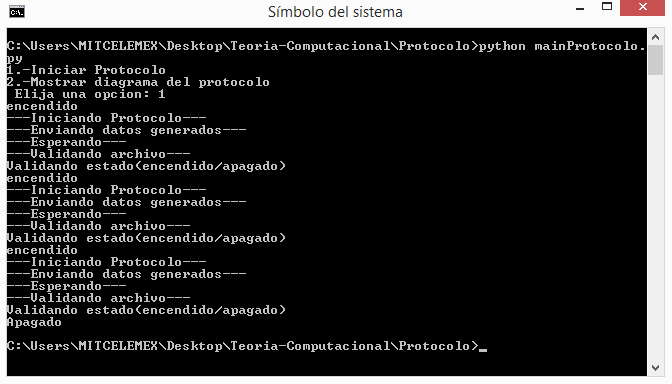
\includegraphics[width=\textwidth, height=9cm]{inicioProtocolo.png}
\label{fig:protocolo}
\caption{iniciar protocolo}
\end{figure}

\begin{figure}[H]
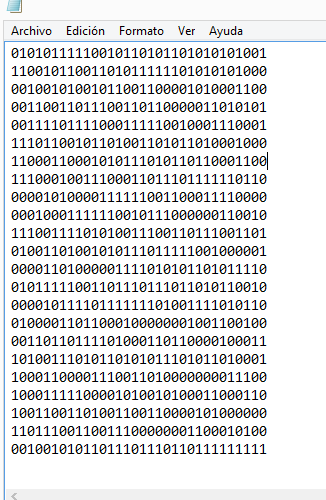
\includegraphics[width=\textwidth, height=9cm]{textoProtocolo.png}
\label{fig:protocoloTexto}
\caption{Cadenas aceptadas por el protocolo}
\end{figure}

\begin{figure}[H]
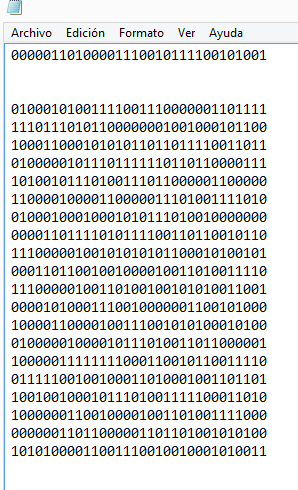
\includegraphics[width=\textwidth, height=9cm]{textoProtocoloFin.png}
\label{fig:protocoloTexto2}
\caption{Cadenas aceptadas por el protocolo}
\end{figure}

\begin{figure}[H]
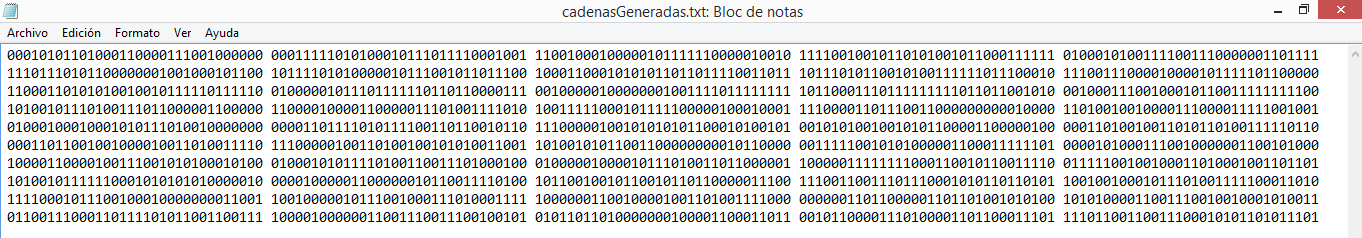
\includegraphics[width=\textwidth, height=9cm]{textoProtocoloGen.png}
\label{fig:protocoloTextoG}
\caption{Ultimas 50 cadenas binarias generadas(Las cadenas est\'an acomodadas en esta imagen de tal forma que se puedan visualizar todas)}
\end{figure}


\begin{figure}[H]
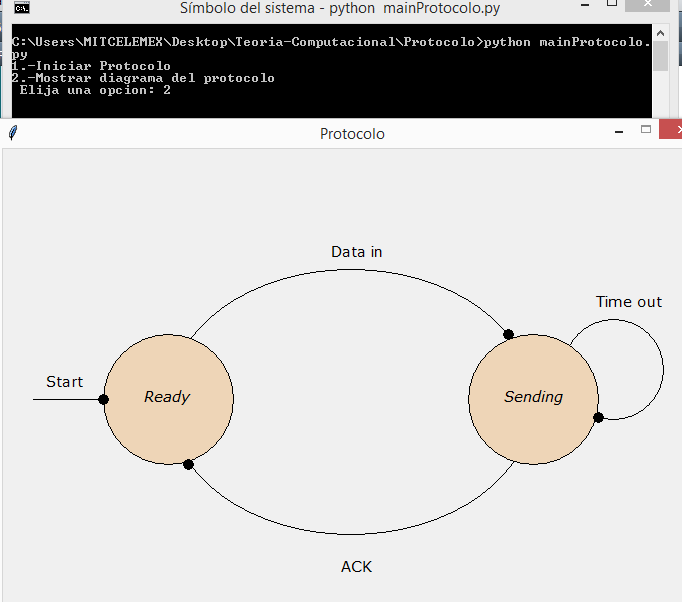
\includegraphics[width=\textwidth, height=15cm]{DiaProtocolo.png}
\label{fig:protocoloDiag}
\caption{Diagrama del protocolo ejecutado desde el programa}
\end{figure}
\newpage
\section{Cadenas terminadas en 01}
\subsection{Descripci\'on}
El programa localiza cada una de las cadenas terminadas en 01, esto se har\'a mediante un aut\'omata no deterministico, tendr\'a un modo para ingresar la cadena manualmente y uno mediante el cual se genere.\\
El aut\'omata que se utilizara ser\'a el siguiente\\
\begin{figure}[H]
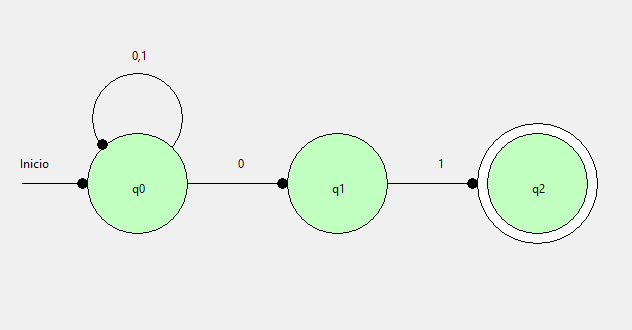
\includegraphics[width=\textwidth, height=6cm]{AND.png}
\label{fig:AND}
\caption{Diagrama del aut\'omata}
\end{figure}

\subsection{c\'odigo}

C\'odigo:DiagramaAND.py\\
\lstset{language=Python, breaklines=true, basicstyle=\footnotesize}
\begin{lstlisting}[frame=single]
from tkinter import *

def mostrarAND():
	ventana =  Tk()
	ventana.geometry("650x500")  #geometry(widthxheight)
	ventana.title("Automata no deterministico")
	ventana.resizable(width=False,height=False)
	AreaDibujo=Canvas(ventana,width=650,height=500)
	AreaDibujo.pack()

	#circulo transicion
	AreaDibujo.create_oval(105,140,195,230)

	#Circulos de estado
	AreaDibujo.create_oval(100,200,200,300,fill="DarkSeaGreen1")
	AreaDibujo.create_oval(300,200,400,300,fill="DarkSeaGreen1")
	AreaDibujo.create_oval(490,190,610,310,fill="white")
	AreaDibujo.create_oval(500,200,600,300,fill="DarkSeaGreen1")

	#lineas de transicion

	AreaDibujo.create_line(35,250,100,250)
	AreaDibujo.create_line(200,250,300,250)
	AreaDibujo.create_line(400,250,490,250)

	#Circulos de sentido

	AreaDibujo.create_oval(90,245,100,255,fill="black")
	AreaDibujo.create_oval(290,245,300,255,fill="black")
	AreaDibujo.create_oval(480,245,490,255,fill="black")
	AreaDibujo.create_oval(110,206,120,216,fill="black")

	#Etiquetas
	inicio=Label(ventana,text="Inicio").place(x=30,y=220)
	q0=Label(ventana,text="q0",background="DarkSeaGreen1").place(x=142,y=245)
	q1=Label(ventana,text="q1",background="DarkSeaGreen1").place(x=342,y=245)
	q2=Label(ventana,text="q2",background="DarkSeaGreen1").place(x=542,y=245)
	cero=Label(ventana,text="0").place(x=248,y=220)
	uno=Label(ventana,text="1").place(x=448,y=220)
	cero_uno=Label(ventana,text="0,1").place(x=142,y=112)

	ventana.mainloop()
\end{lstlisting}
\vspace{1 cm}
\subsection{Pruebas}
Se mostrara la prueba del diagrama.\\
\begin{figure}[H]
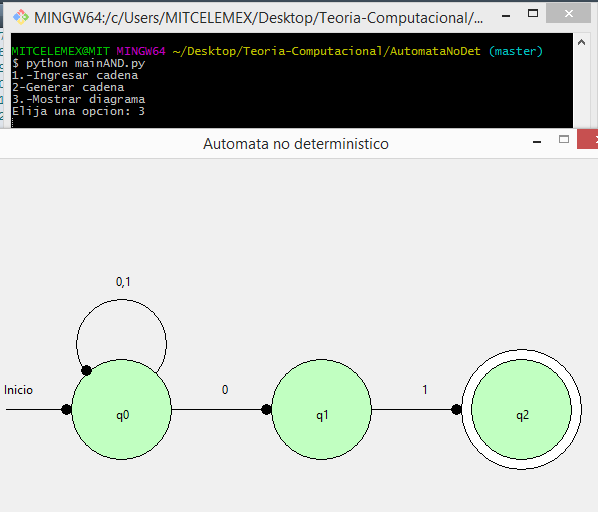
\includegraphics[width=\textwidth, height=10cm]{diagAND.png}
\label{fig:diagAND}
\caption{Diagrama del aut\'omata en ejecuci\'on}
\end{figure}
\newpage

\begin{thebibliography}{X}
\bibitem{uno} \textsc{Biograf\'ias y Vida},
\textit{William Shakespeare}, url: http://www.biografiasyvidas.com/biografia/s/shakespeare.html

\bibitem{Dan} \textsc{	HOPCROFT JOHN, MOTWANI RAJEEV},
<<Introduction to Automata Theory,
Languages and Computation>>,
\textit{Addison Wesley},2008
\end{thebibliography}

\end{document}